\question{3}
\label{q:pregunta3}

% Descripción de la pregunta
Suponga que debido a una falla en la maquinaria de procesamiento, la capacidad de procesamiento en el periodo 3 se reduce a la mitad. Resuelva nuevamente el modelo bajo esta condición y compare los resultados con la planificación original.

\answer

\subsection*{Análisis Comparativo: Impacto de la Falla Técnica}

Hemos resuelto el modelo considerando una reducción del 50\% en la capacidad de procesamiento durante el periodo 3. A continuación presentamos una comparación entre la planificación original y la planificación bajo esta nueva restricción.

\subsubsection*{Planificación de Producción y Procesamiento}

\begin{table}[H]
    \centering
    \caption{Comparación de producción y satisfacción de demanda entre escenario base y falla}
    \label{tab:comparativa_produccion}
    \resizebox{\textwidth}{!}{
        \csvreader[
            tabular=cccccccc,
            table head=\toprule \textbf{Periodo} & \textbf{Caso} & \textbf{\begin{tabular}[c]{@{}c@{}}Ropa buen\\estado (kg)\end{tabular}} & \textbf{\begin{tabular}[c]{@{}c@{}}Ropa mal\\estado (kg)\end{tabular}} & \textbf{\begin{tabular}[c]{@{}c@{}}Género\\utilizado (kg)\end{tabular}} & \textbf{\begin{tabular}[c]{@{}c@{}}Prendas\\producidas\end{tabular}} & \textbf{\begin{tabular}[c]{@{}c@{}}Demanda\\satisfecha\end{tabular}} & \textbf{\begin{tabular}[c]{@{}c@{}}Demanda\\insatisfecha\end{tabular}} \\\midrule,
            command=\ifnum\pdfstrcmp{#1}{Total}=0 \textbf{#1} & \textbf{#2} & $\mathbf{#3}$ & $\mathbf{#4}$ & $\mathbf{#5}$ & $\mathbf{#6}$ & $\mathbf{#7}$ & $\mathbf{#8}$ \else #1 & #2 & $#3$ & $#4$ & $#5$ & $#6$ & $#7$ & $#8$ \fi,
            late after line=\\,
            table foot=\bottomrule,
            respect dollar=false,
            respect percent=false
        ]{resources/pregunta3/tabla_comparativa_produccion.csv}{}{}
    }
\end{table}

\subsubsection*{Impacto en la producción y satisfacción de demanda}

\begin{figure}[H]
    \centering
    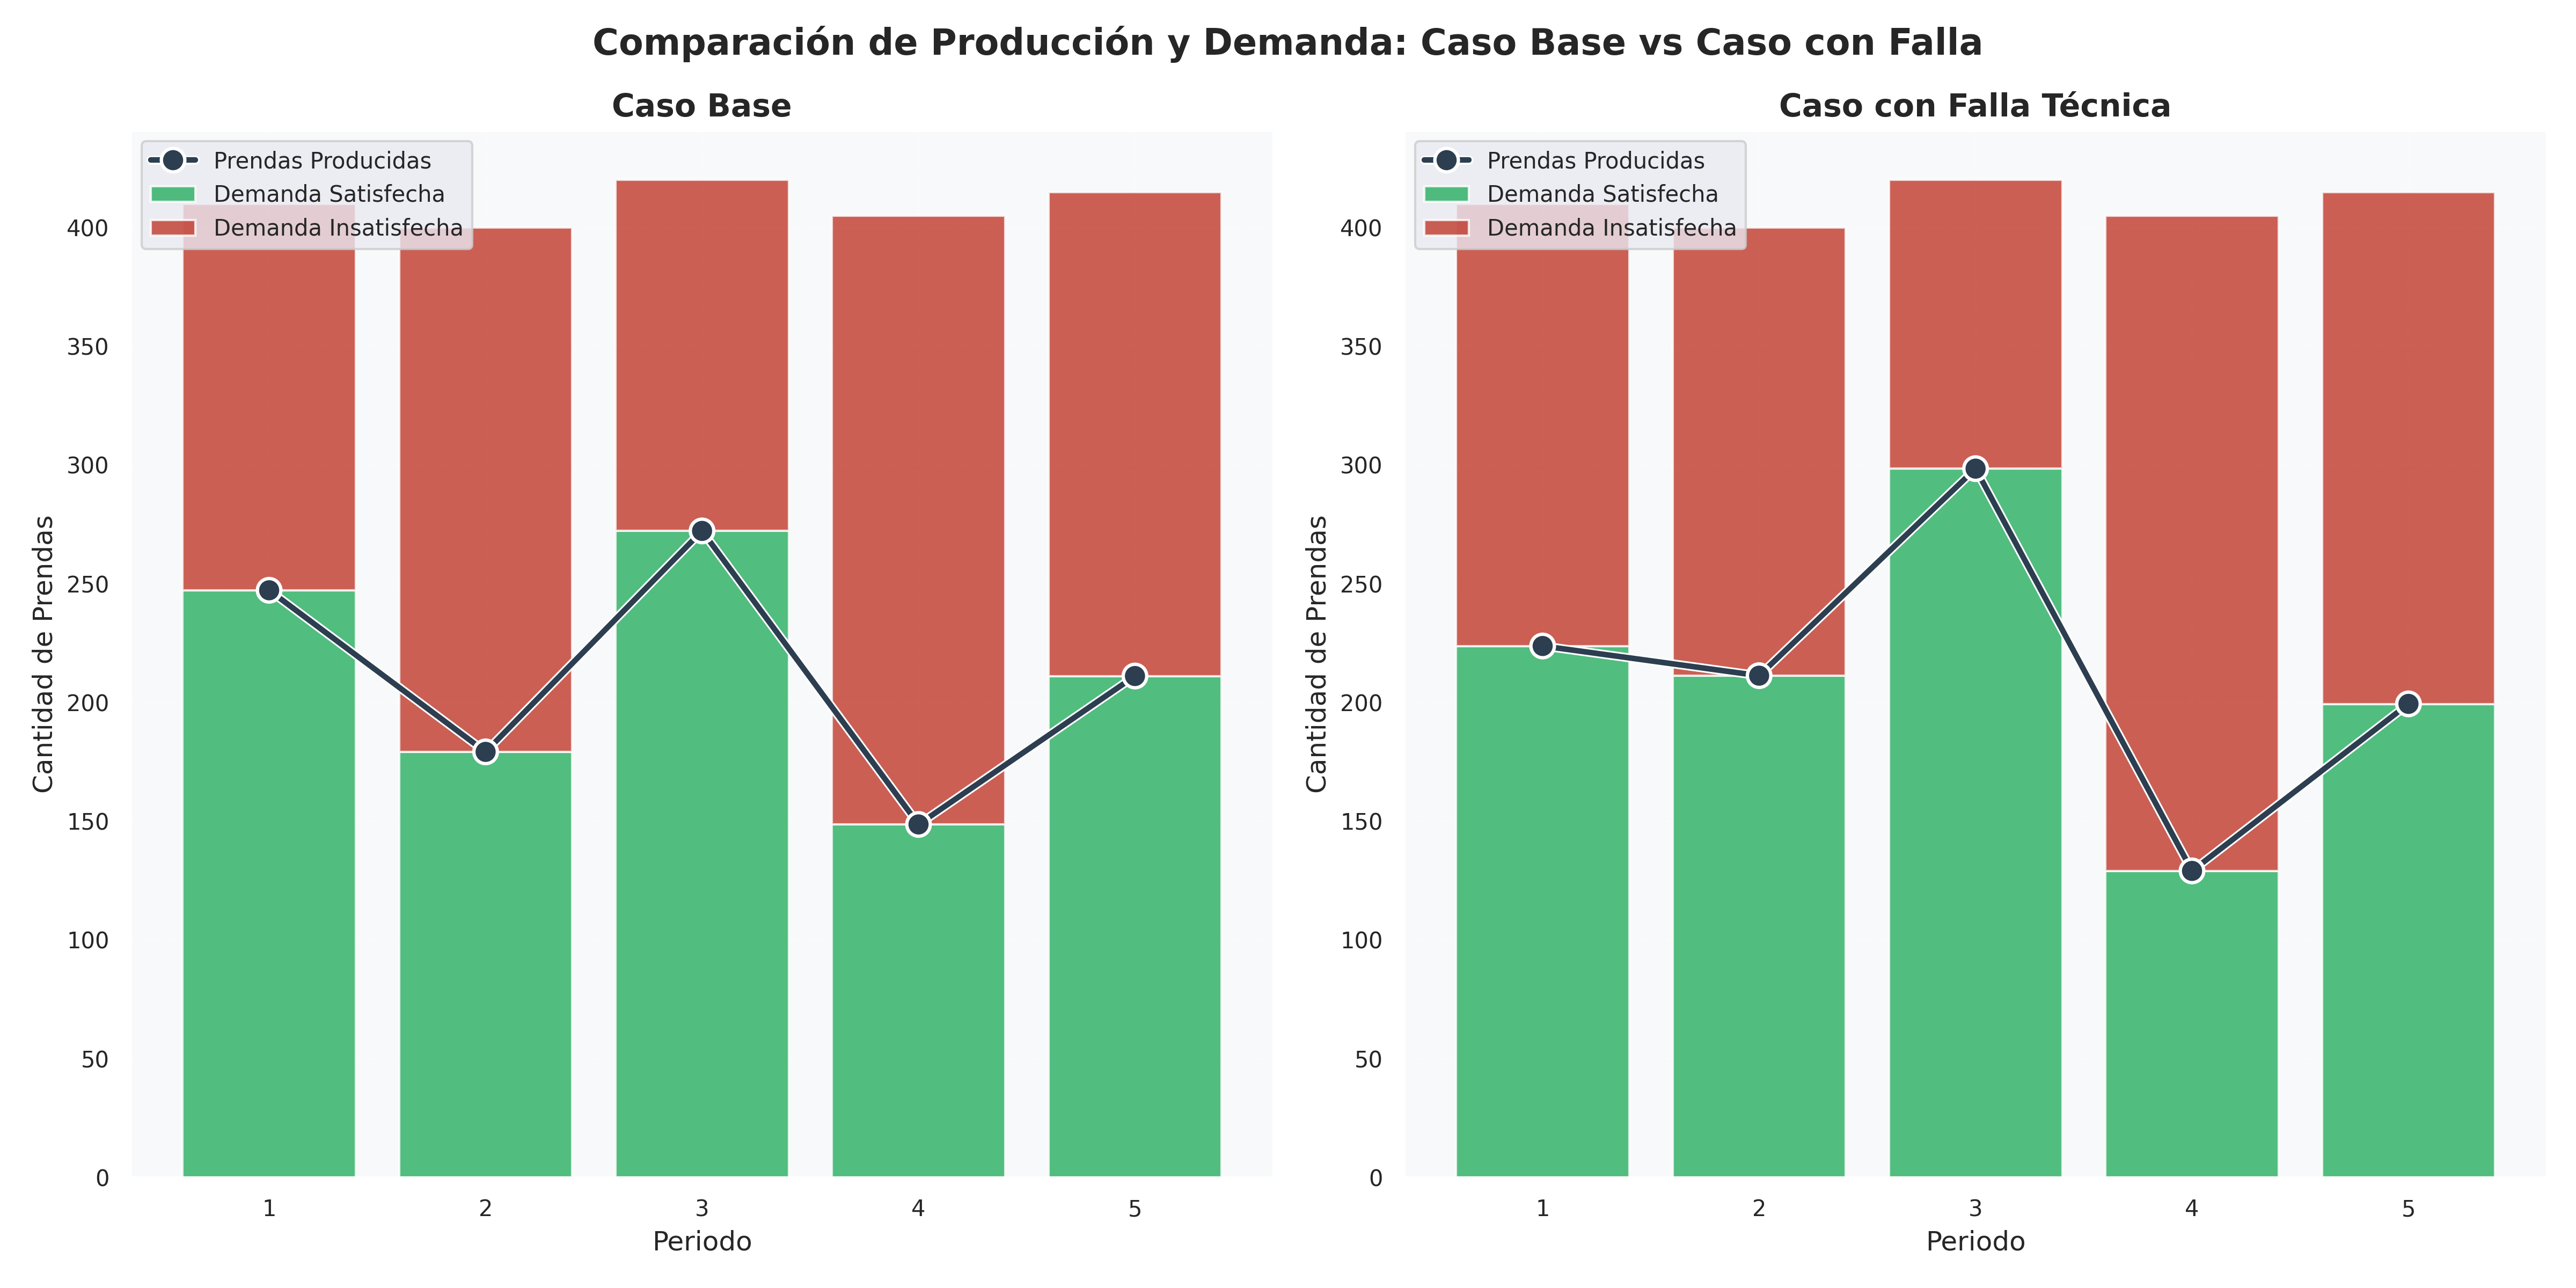
\includegraphics[width=0.9\textwidth]{resources/pregunta3/grafico_comparativo_produccion_demanda.png}
    \caption{Comparación de la producción y satisfacción de demanda entre escenario base y escenario con falla}
    \label{fig:comparativa_produccion}
\end{figure}

\subsubsection*{Comparación de costos}

\begin{figure}[H]
    \centering
    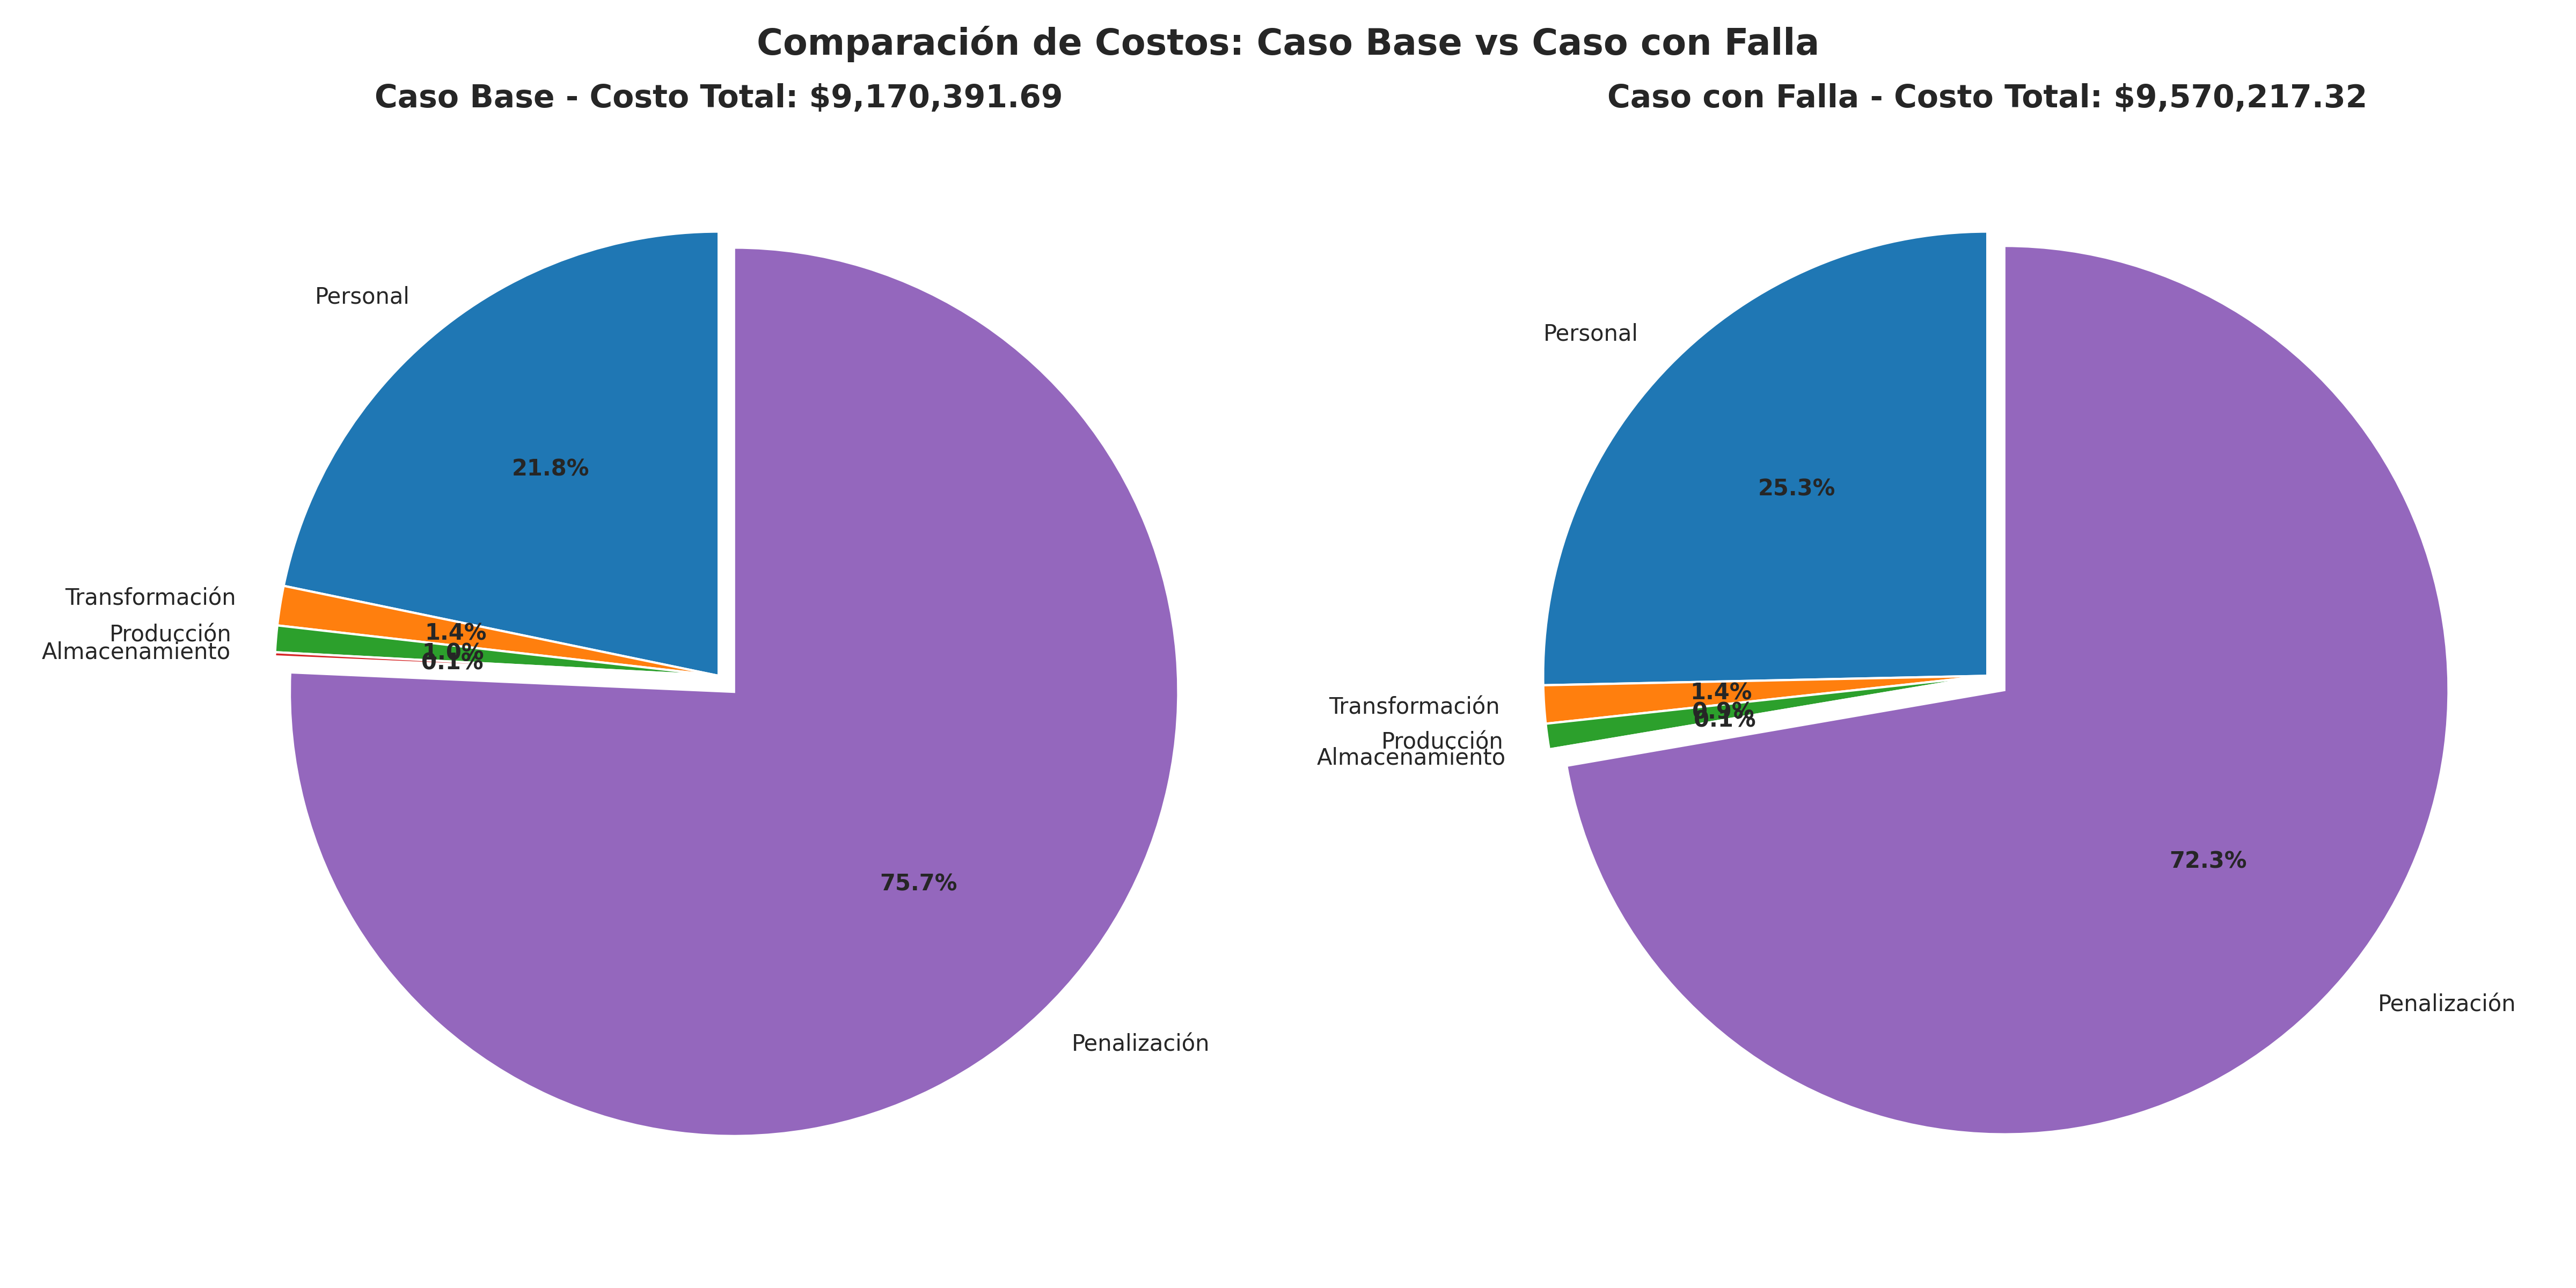
\includegraphics[width=0.9\textwidth]{resources/pregunta3/grafico_comparativo_costos.png}
    \caption{Comparación de la distribución de costos entre escenario base y escenario con falla}
    \label{fig:comparativa_costos}
\end{figure}

\subsubsection*{Inventarios por periodo}

\begin{table}[H]
    \centering
    \caption{Comparación de inventarios entre escenario base y falla}
    \label{tab:comparativa_inventarios}
    \resizebox{\textwidth}{!}{
        \csvreader[
            tabular=cccccccc,
            table head=\toprule \textbf{Periodo} & \textbf{Caso} & \textbf{\begin{tabular}[c]{@{}c@{}}Inv. ropa\\buen estado (kg)\end{tabular}} & \textbf{\begin{tabular}[c]{@{}c@{}}Inv. ropa\\mal estado (kg)\end{tabular}} & \textbf{\begin{tabular}[c]{@{}c@{}}Inv. género\\(kg)\end{tabular}} & \textbf{\begin{tabular}[c]{@{}c@{}}Almacenamiento\\total (kg)\end{tabular}} & \textbf{\begin{tabular}[c]{@{}c@{}}\% Capacidad\\utilizada\end{tabular}} \\\midrule,
            command=#1 & #2 & $#3$ & $#4$ & $#5$ & $#6$ & $#7$,
            late after line=\\,
            table foot=\bottomrule,
            respect dollar=false,
            respect percent=false
        ]{resources/pregunta3/tabla_comparativa_inventarios.csv}{}{}
    }
\end{table}

\subsubsection*{Recursos humanos y utilización}

\begin{figure}[H]
    \centering
    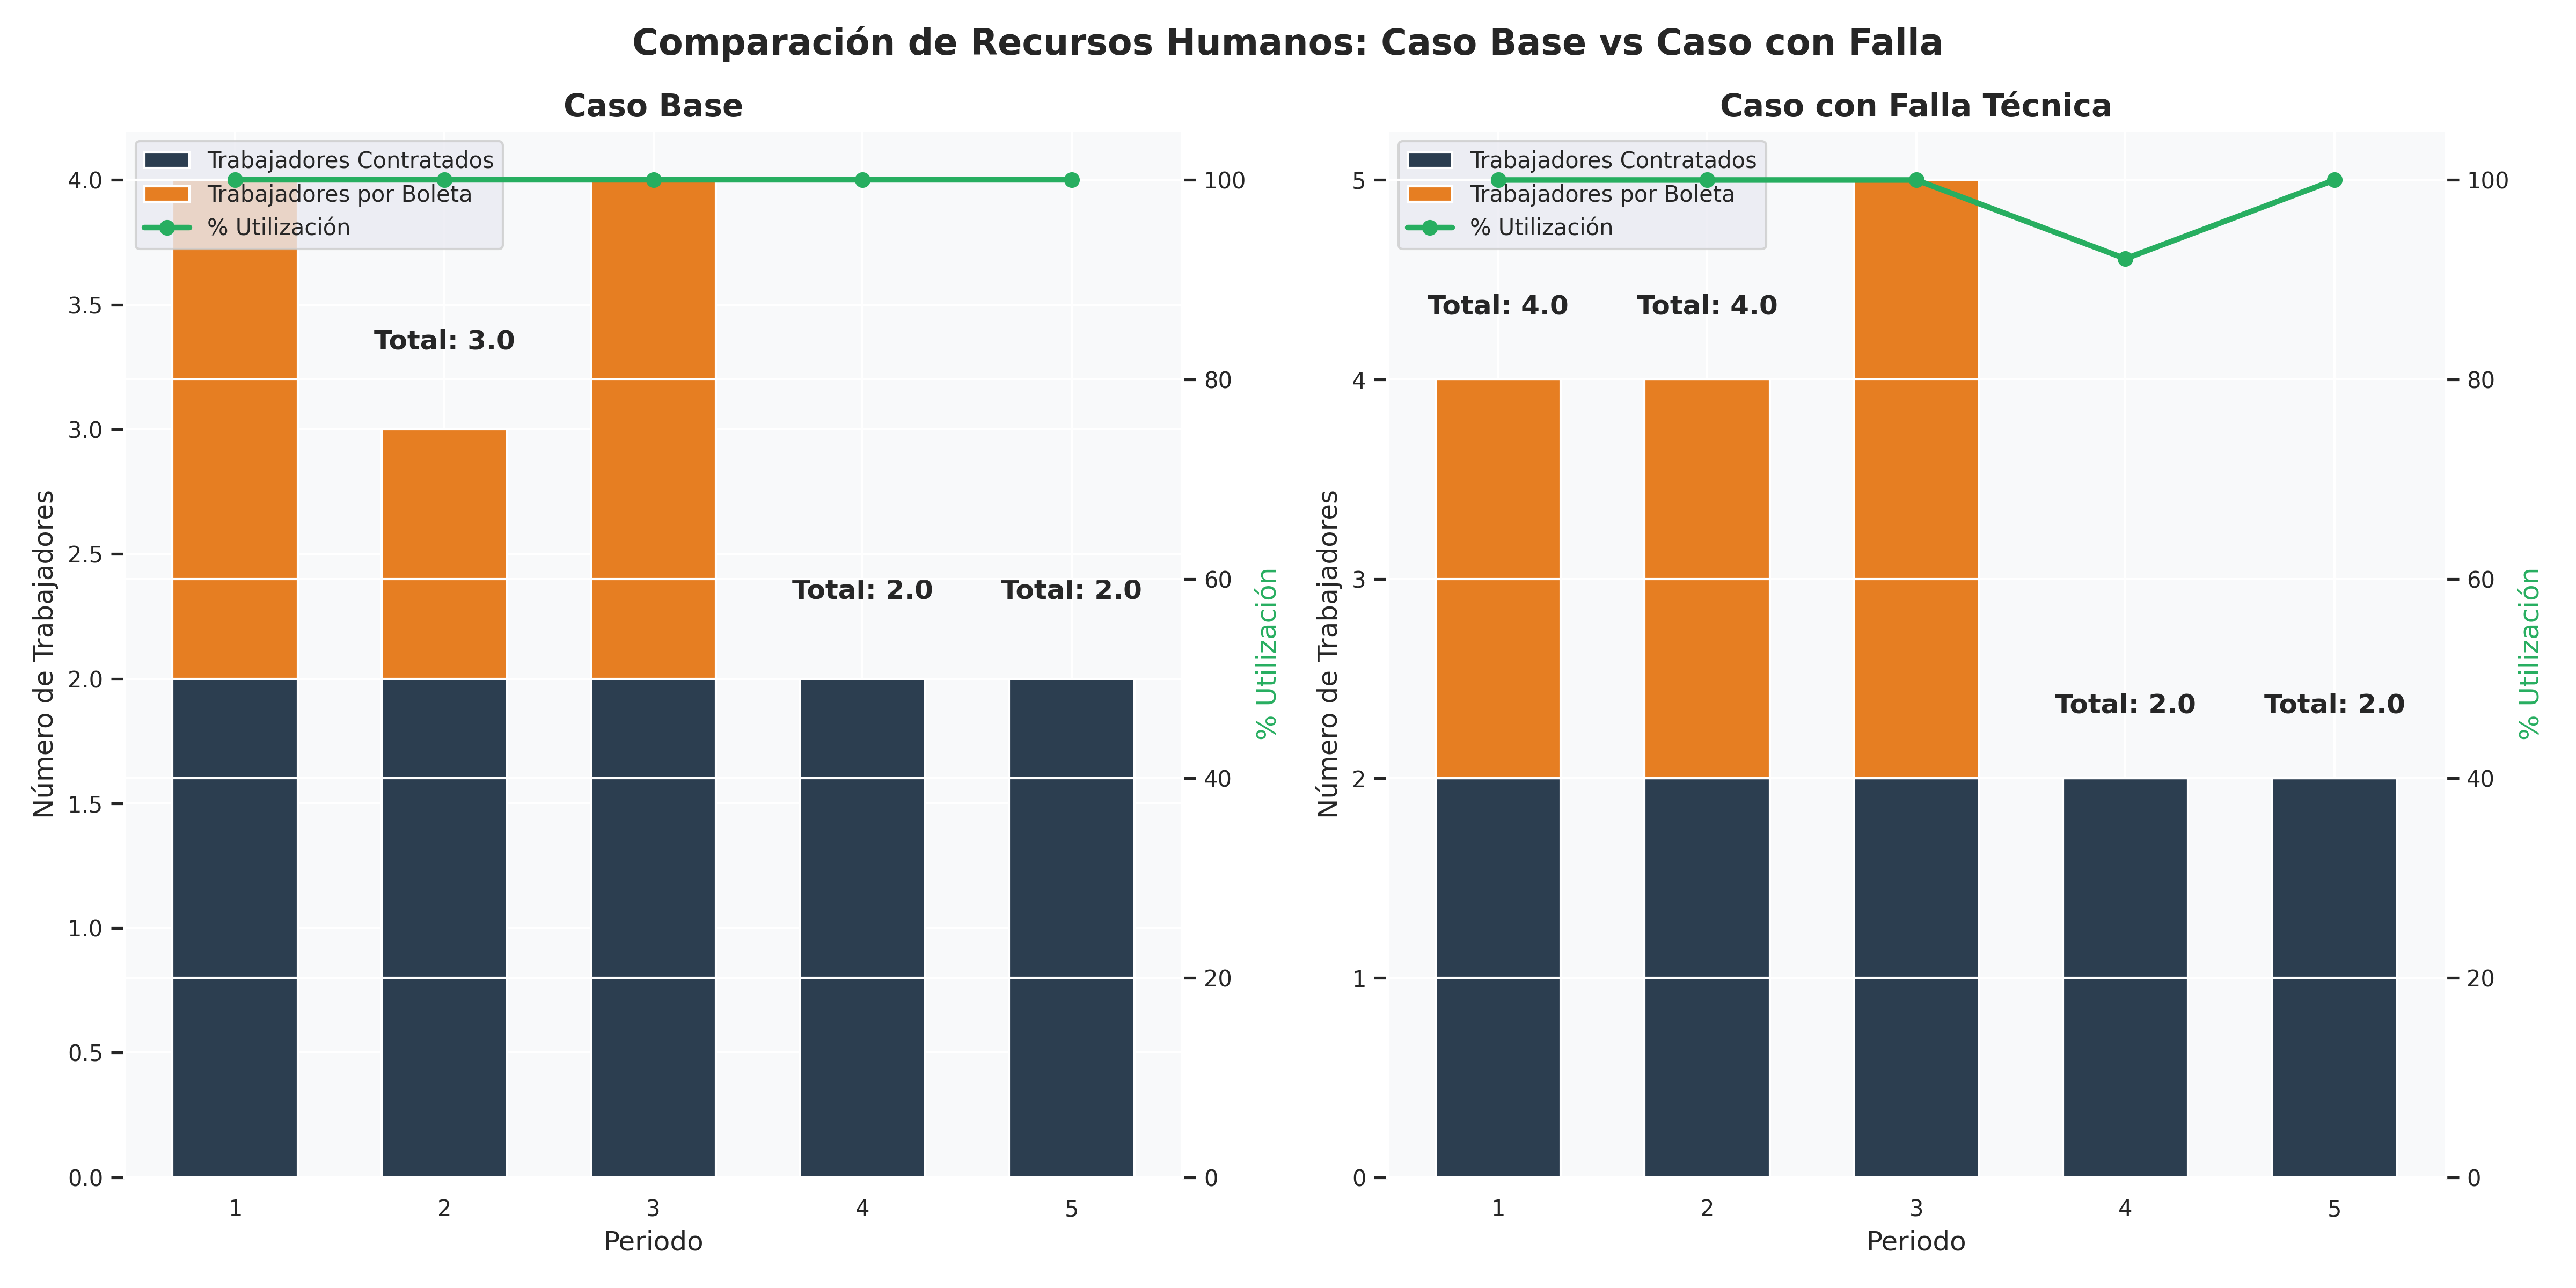
\includegraphics[width=0.9\textwidth]{resources/pregunta3/grafico_comparativo_recursos_humanos.png}
    \caption{Comparación de recursos humanos entre escenario base y escenario con falla}
    \label{fig:comparativa_rrhh}
\end{figure}

\begin{table}[H]
    \centering
    \caption{Comparación de recursos humanos entre escenario base y falla}
    \label{tab:comparativa_rrhh}
    \resizebox{\textwidth}{!}{
        \csvreader[
            tabular=ccccccccc,
            table head=\toprule \textbf{Periodo} & \textbf{Caso} & \textbf{\begin{tabular}[c]{@{}c@{}}Trabajadores\\contratados\end{tabular}} & \textbf{\begin{tabular}[c]{@{}c@{}}Trabajadores\\por boleta\end{tabular}} & \textbf{\begin{tabular}[c]{@{}c@{}}Total\\trabajadores\end{tabular}} & \textbf{\begin{tabular}[c]{@{}c@{}}Horas\\disponibles\end{tabular}} & \textbf{\begin{tabular}[c]{@{}c@{}}Horas\\utilizadas\end{tabular}} & \textbf{\begin{tabular}[c]{@{}c@{}}\% Utilización\end{tabular}} \\\midrule,
            command=\ifnum\pdfstrcmp{#1}{Total}=0 \textbf{#1} & \textbf{#2} & $\mathbf{#3}$ & $\mathbf{#4}$ & $\mathbf{#5}$ & $\mathbf{#6}$ & $\mathbf{#7}$ & $\mathbf{#8}$ \else #1 & #2 & $#3$ & $#4$ & $#5$ & $#6$ & $#7$ & $#8$ \fi,
            late after line=\\,
            table foot=\bottomrule,
            respect dollar=false,
            respect percent=false
        ]{resources/pregunta3/tabla_comparativa_rrhh.csv}{}{}
    }
\end{table}

\subsubsection*{Capacidad de procesamiento}

\begin{figure}[H]
    \centering
    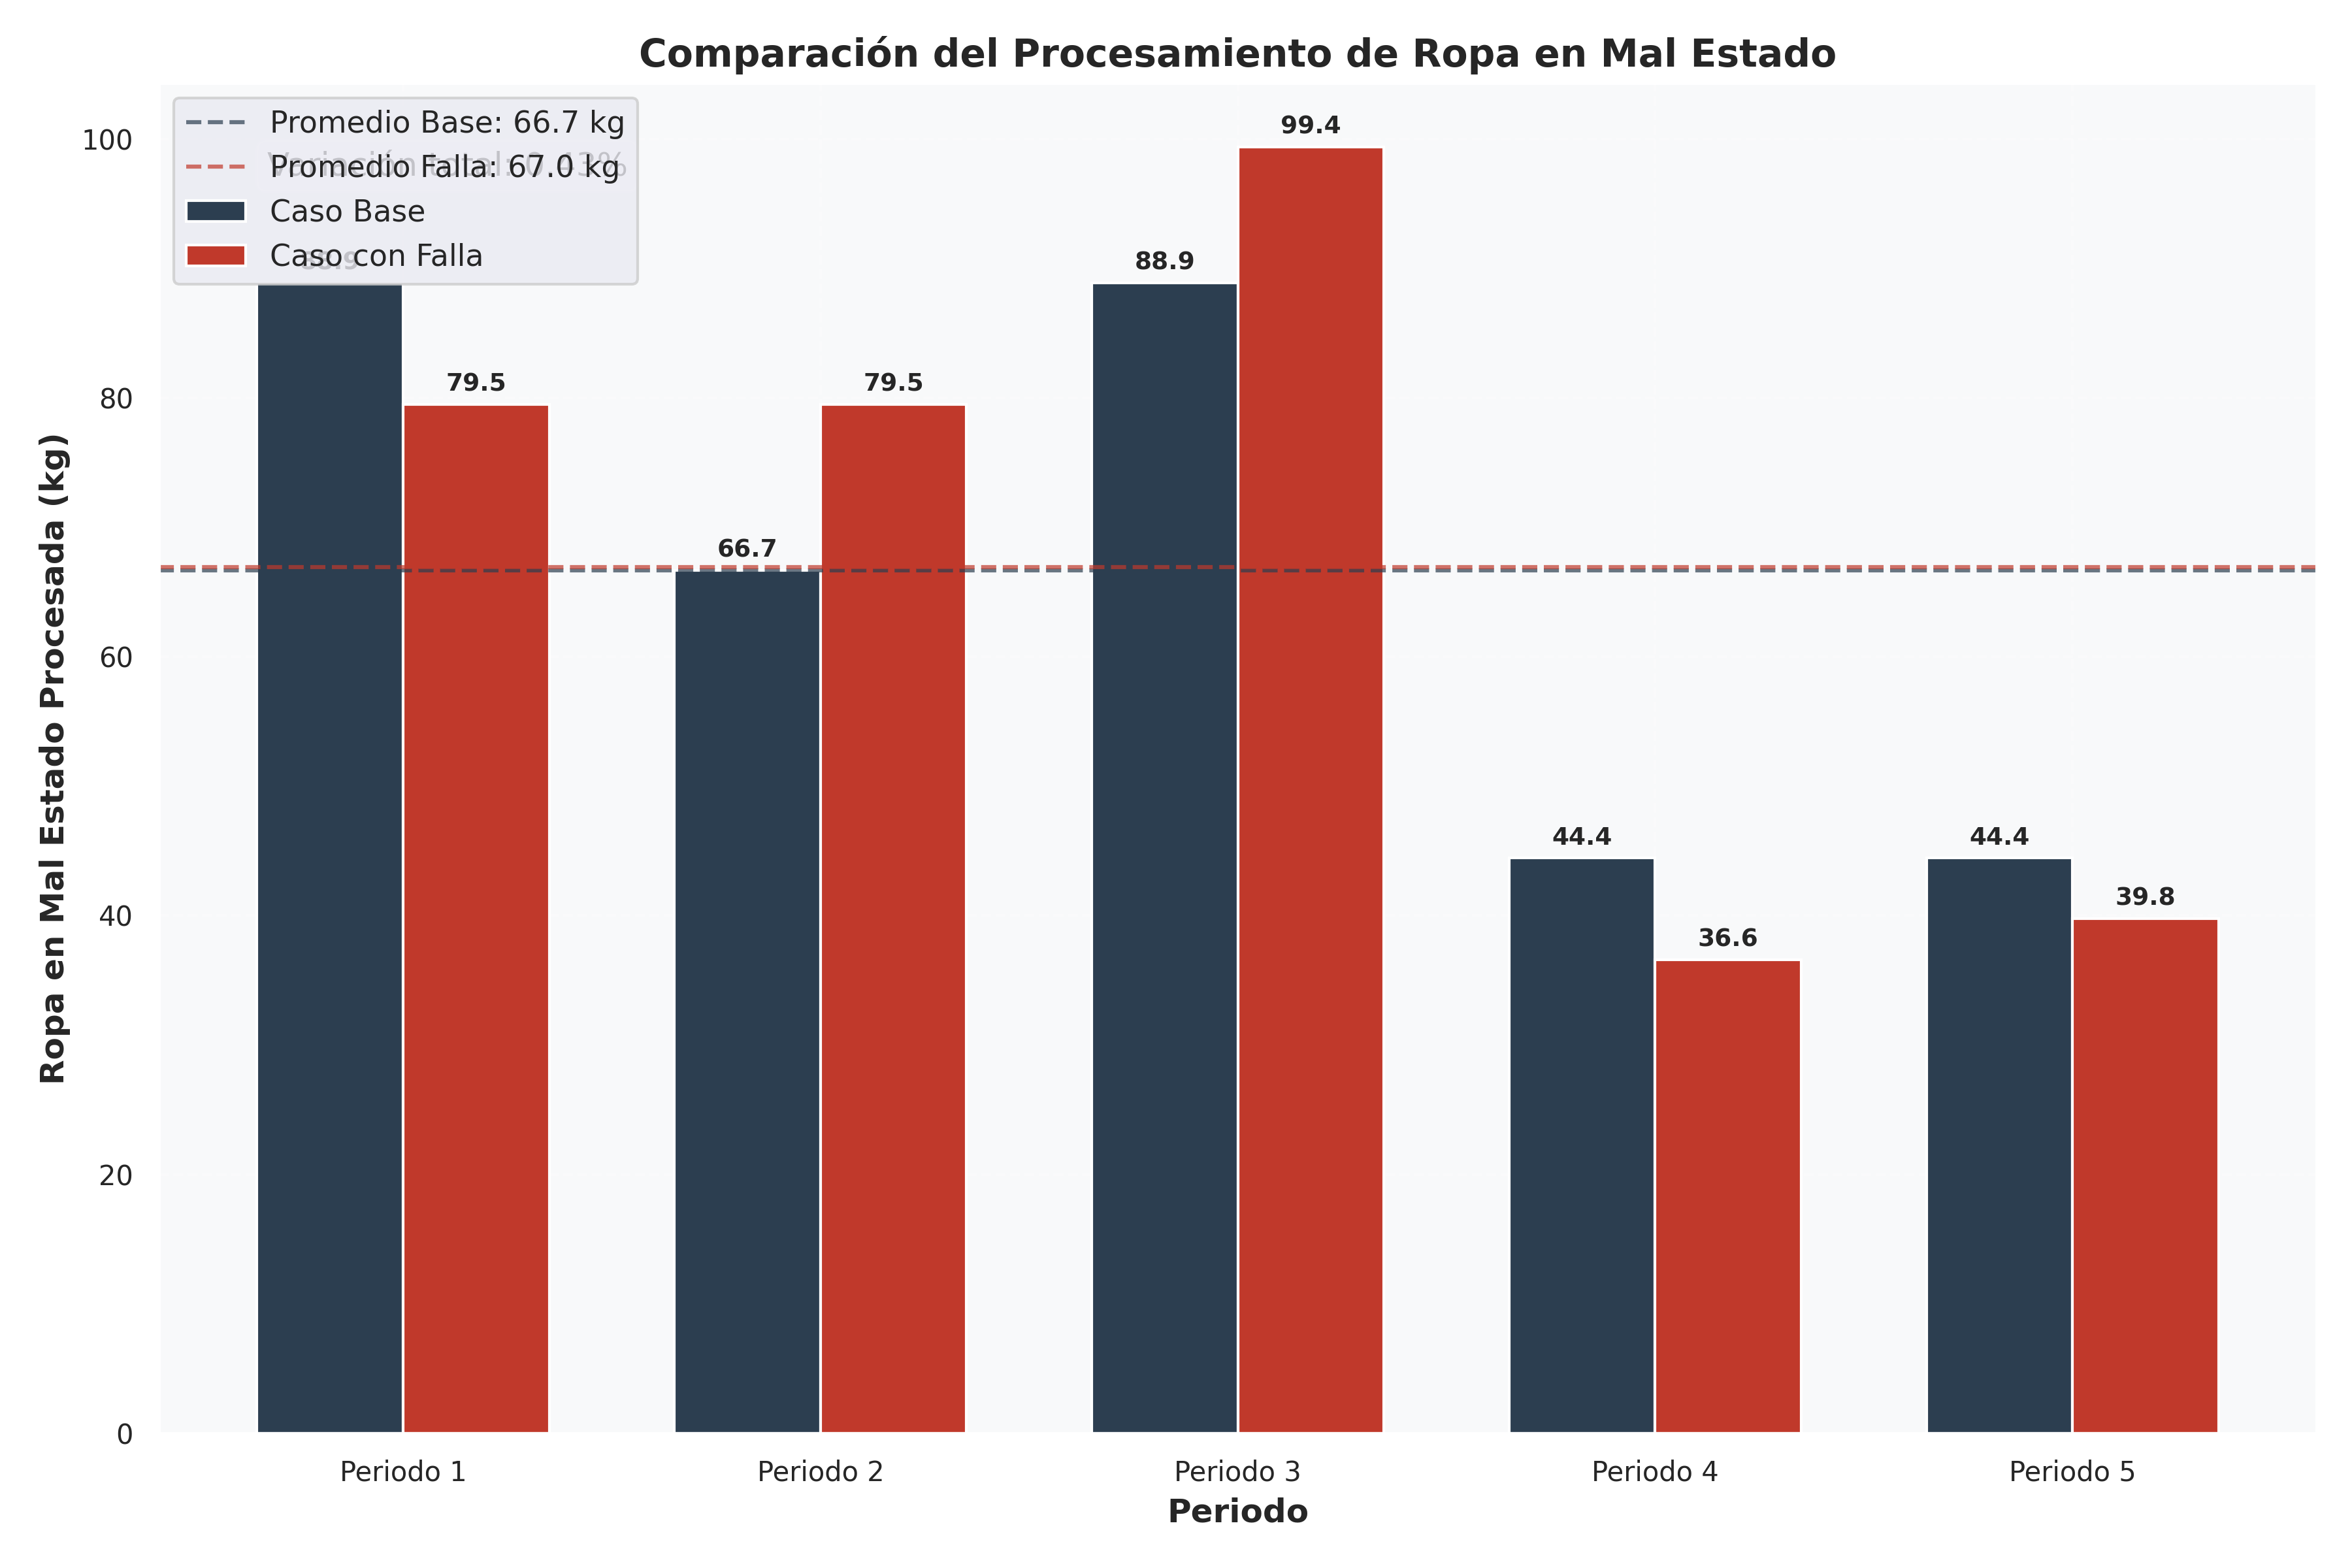
\includegraphics[width=0.9\textwidth]{resources/pregunta3/grafico_comparativo_procesamiento.png}
    \caption{Comparación de la capacidad de procesamiento entre escenario base y escenario con falla}
    \label{fig:comparativa_procesamiento}
\end{figure}

\subsection*{Análisis del Impacto de la Falla}

La reducción de la capacidad de procesamiento en el periodo 3 ha generado los siguientes efectos en la planificación óptima:

\begin{itemize}
    \item \textbf{Redistribución de la producción:} Se observa un desplazamiento de la producción hacia otros periodos para compensar la reducción de capacidad.
    \item \textbf{Aumento en costos totales:} El costo total aumenta debido a la necesidad de ajustar la planificación y contratar más trabajadores por boleta.
    \item \textbf{Mayor dotación de personal:} Se requieren 2 trabajadores adicionales por boleta para compensar la falla, aumentando los costos laborales.
    \item \textbf{Cambios en niveles de inventario:} Los niveles de inventario se ajustan para compensar la reducción en la capacidad productiva.
\end{itemize}

\subsection*{Conclusiones}

La falla en la maquinaria durante el periodo 3 genera un impacto significativo en la planificación óptima. A pesar de la reducción de capacidad, el modelo logra mantener niveles similares de producción y satisfacción de demanda mediante la redistribución de recursos. Se recomienda implementar medidas preventivas de mantenimiento para evitar este tipo de situaciones, ya que el impacto económico es considerable.
